\section{Detection of the interaction}

\subsection{Contexte}
\addtocounter{framenumber}{-1}

\sframe{Detecting the influenza-pneumococcus interaction}{
	Numerous studies but no gold standard
	
	\begin{enumerate}
		\item Regression models
		\medskip
		\item Dynamical models
	\end{enumerate}
	
	\bigskip
	\visible<2>{
	\begin{center}
	\head{Are these methods adequate to detect such an interaction?}\\
	\bigskip
	
\includegraphics[scale=.06]{figures/illustrations/undraw_not_found_60pq.png}
	\end{center}
	}
}


\sframe{Study design}{
	\only<1>{
	\begin{center}
	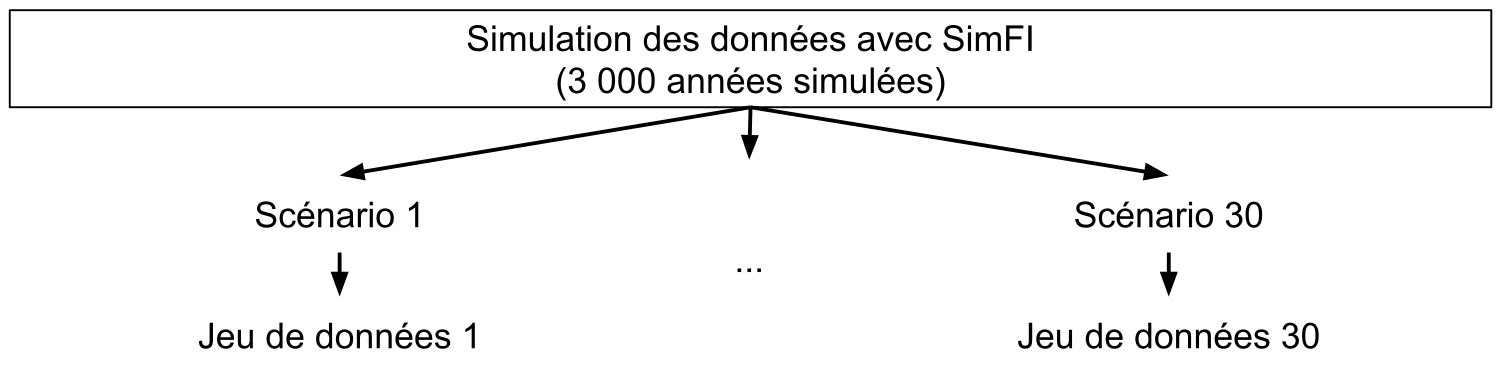
\includegraphics[width=\textwidth]{figures/analysis/principe_etude_sim.png}
	\end{center}
	}
	\only<2>{
	\begin{center}
	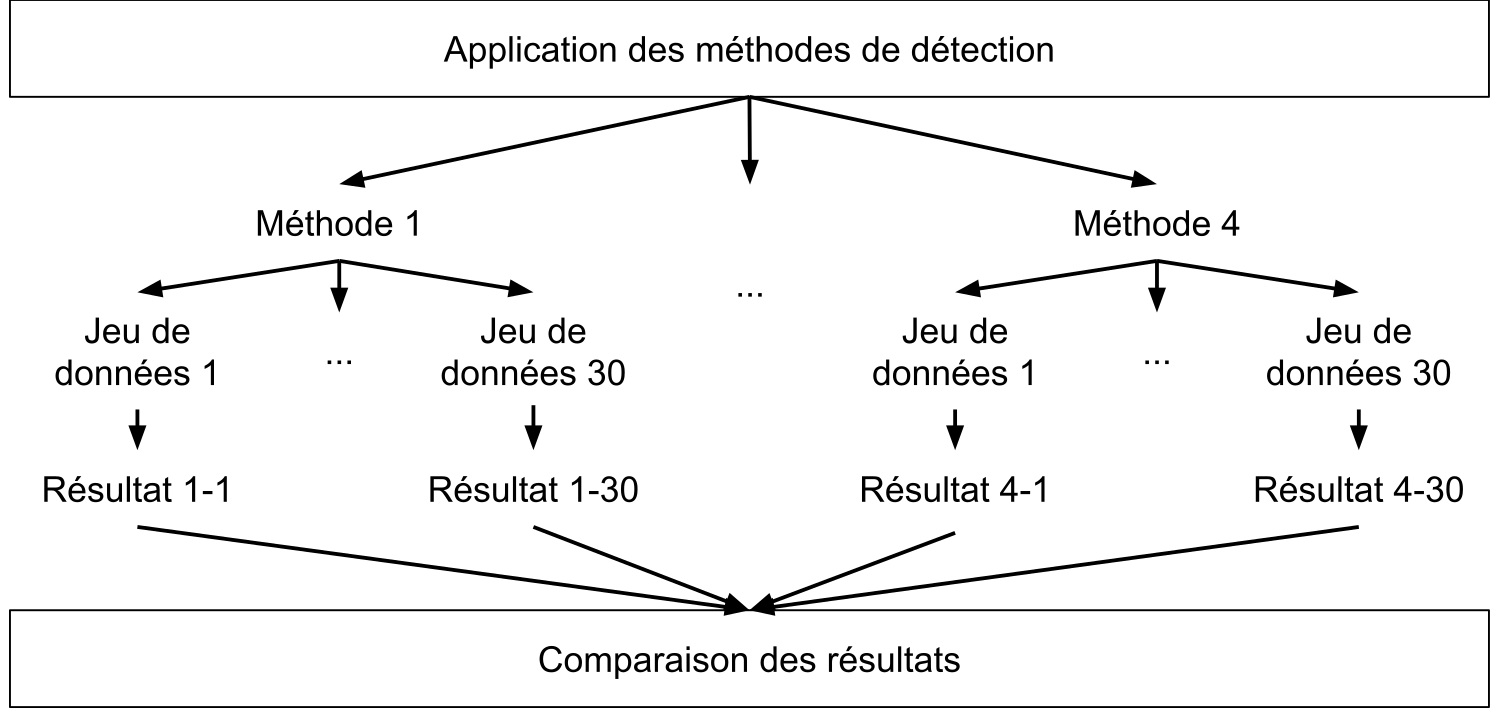
\includegraphics[width=\textwidth]{figures/analysis/principe_etude_meth.png}
	\end{center}
	}
}



\subsection{Modèles}

\sframe{Regression model}{
	\begin{eqnarray*}
		F({\color{red}I_t}) &=& a + b{\color{red}G_{t+i}} + c\cos{\dfrac{2\pi t}{52}} + d\sin{\dfrac{2\pi t}{52}} + \epsilon_t
	\end{eqnarray*}
	
	\bigskip
	
%	\begin{columns}
%	\begin{column}{.6\textwidth}
	\only<1>{
	\begin{table}
	\begin{tabular}{cl}
  		$F$ & transformation\\
  		& (linear, Poisson, or\\
  		& negative binomiale)\\
  		$I_t$ & pneumococcal infections\\
  		$G_{t+i}$ & influenza infections\\
  		$t$ & week\\
  		$i$ & time lag
  	\end{tabular}
  	\end{table}
  	}
%	\end{column}
%	
%	\begin{column}{.5\textwidth}
	\only<2>{
	\begin{center}
	$\rightarrow$ 1~134~000 regressions\\
	
	\bigskip
	
	\head{Results comparison}\\
	Student t-test: $t = \dfrac{\hat{b}}{SE_b}$
	
	\bigskip
	
	\head{Softwares and computing resources}\\
	\bigskip
	
\includegraphics[height=.5cm]{figures/logos/Rlogo.png}
	
\includegraphics[height=.5cm]{figures/logos/openmole.png}
	
\includegraphics[height=.5cm]{figures/logos/egi.png}
	\end{center}
	}
	
%	\end{column}
%	\end{columns}
}


\sframe{Pneumococcus transmission model}{
	\begin{center}
	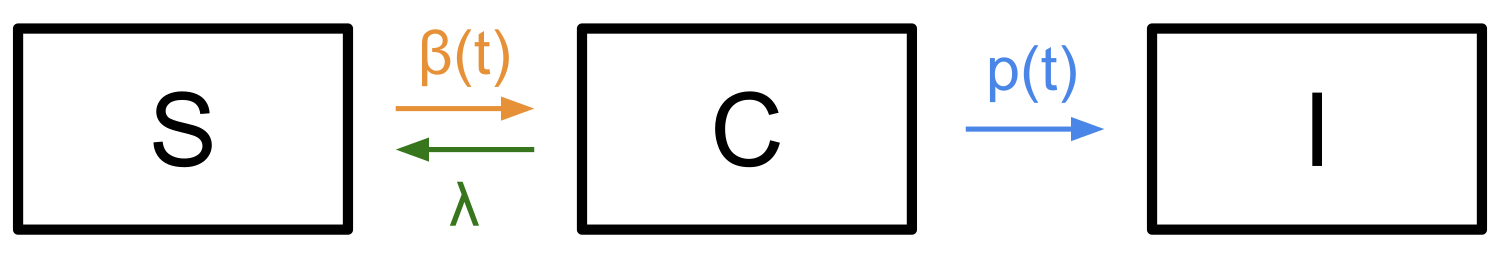
\includegraphics[width=.75\textwidth]{figures/analysis/modele_lulla.png}
	\end{center}
		
	\begin{columns}
	\begin{column}{.6\textwidth}
		\begin{eqnarray*}
			\left\{
			\begin{array}{lcl}
				\dv{S}{t} & = & \lambda C(t) -\beta(t)\dfrac{S(t)C(t)}{N} \\
				\tmspace{1mu}&& \\
				\dv{C}{t} & = & -\lambda C(t) + \beta(t)\dfrac{S(t)C(t)}{N} \\
				\tmspace{1mu}&& \\
				\dv{I}{t} & = & p(t)C(t)
			\end{array}
			\right.
		\end{eqnarray*}
	\end{column}
	
	\begin{column}{.5\textwidth}	
		\begin{eqnarray*}
			\left\{
			\begin{array}{lcl}
				\beta(t) & = & \beta_{0}(1 + \xi\times G(t)) \\
				\tmspace{1mu}&& \\
				p(t) & = & p_{0}(1 + \pi\times G(t))
			\end{array}
			\right.
		\end{eqnarray*}
	\end{column}
	\end{columns}
	
	\bigskip
	
	\begin{center}
	4 parameters to estimate: $\beta_0$, $\xi$, $p_0$ et $\pi$.
	\end{center}
	
	\begin{flushright}
	\refs{Opatowski}{2013}{}
	\end{flushright}
}


%\sframe{Résultats des régressions de Poisson}
%	\begin{center}
%		\vspace{-.2cm}
%		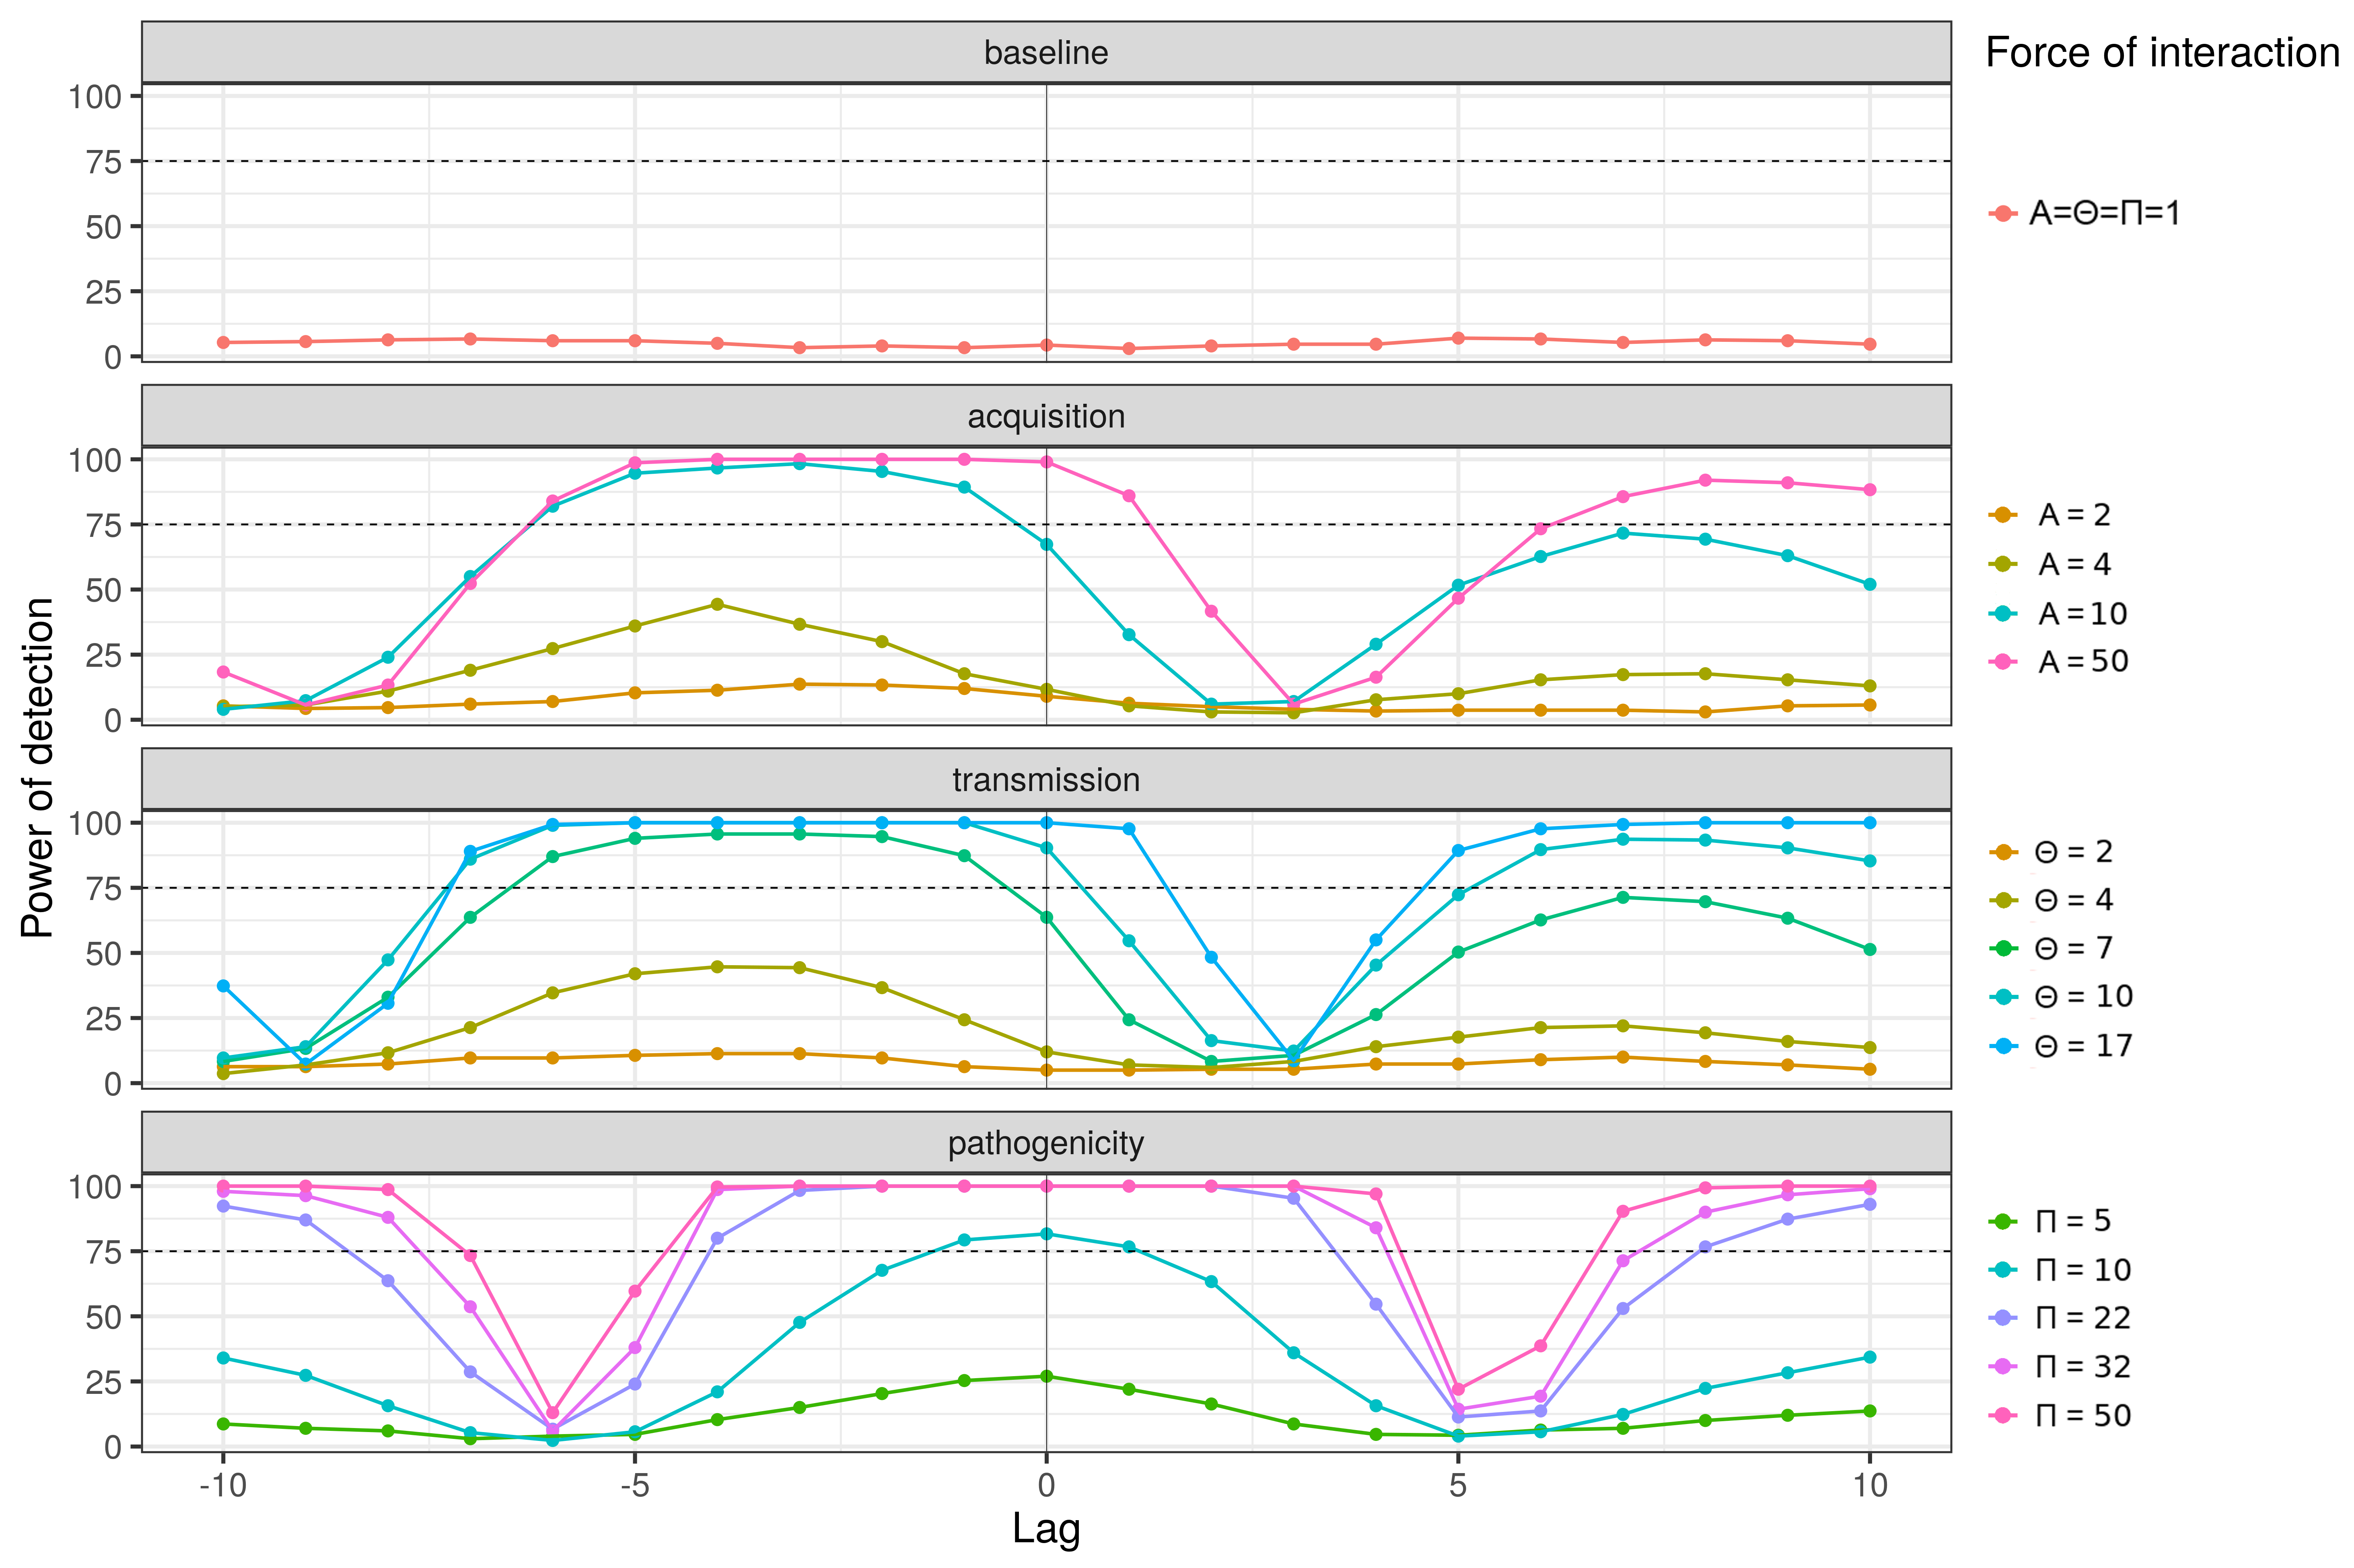
\includegraphics[width=\textwidth]{figures/analysis/plot_power_article_prixThese.png}
%	\end{center}
%}


\sframe{Parameter estimation}{
	$\rightarrow$ 36~000 estimations and their confidence intervals\\
	
	\bigskip
	
	\head{Likelihood maximisation}
	
	\begin{itemize}
		\item Poisson likelihood
		\medskip
		\item Estimation: NSGA-2 algorithm \refs{Deb}{2002}{}

		\medskip
		\item Confidence intervals : profiled likelihood on the OpenMOLE platform \refs{Reuillon}{2015}{}
	\end{itemize}
	
	\begin{center}
	\head{Softwares and computing resources}\\
	\bigskip
	
\includegraphics[height=.5cm]{figures/logos/Rlogo.png}
	
\includegraphics[height=.5cm]{figures/logos/openmole.png}
	
\includegraphics[height=.5cm]{figures/logos/egi.png}
	\end{center}
}

\sframe{Profile example}{
	\begin{center}
		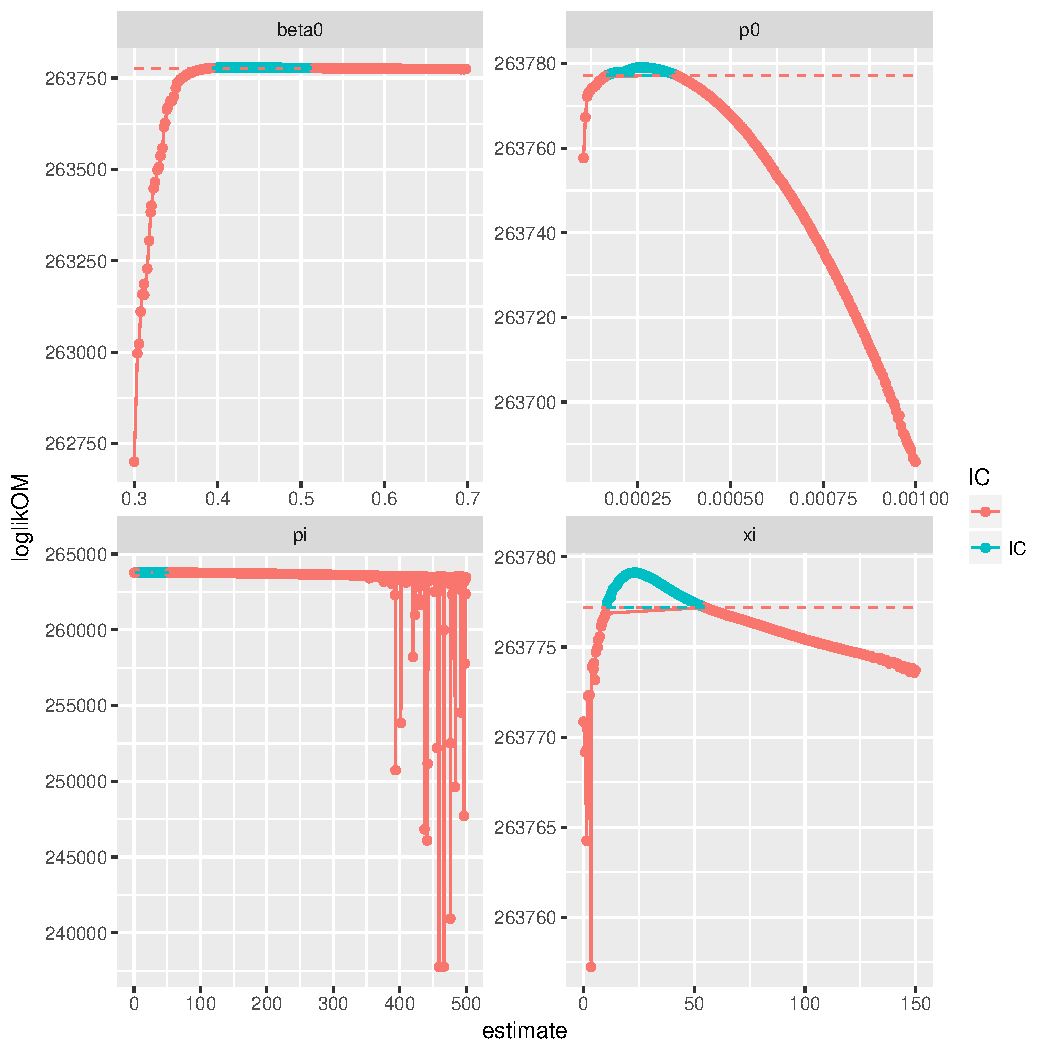
\includegraphics[width=\textwidth]{figures/analysis/profiles.pdf}
	\end{center}
}


%\sframe{Estimation des paramètres d'interaction du modèle}
%	\begin{center}
%	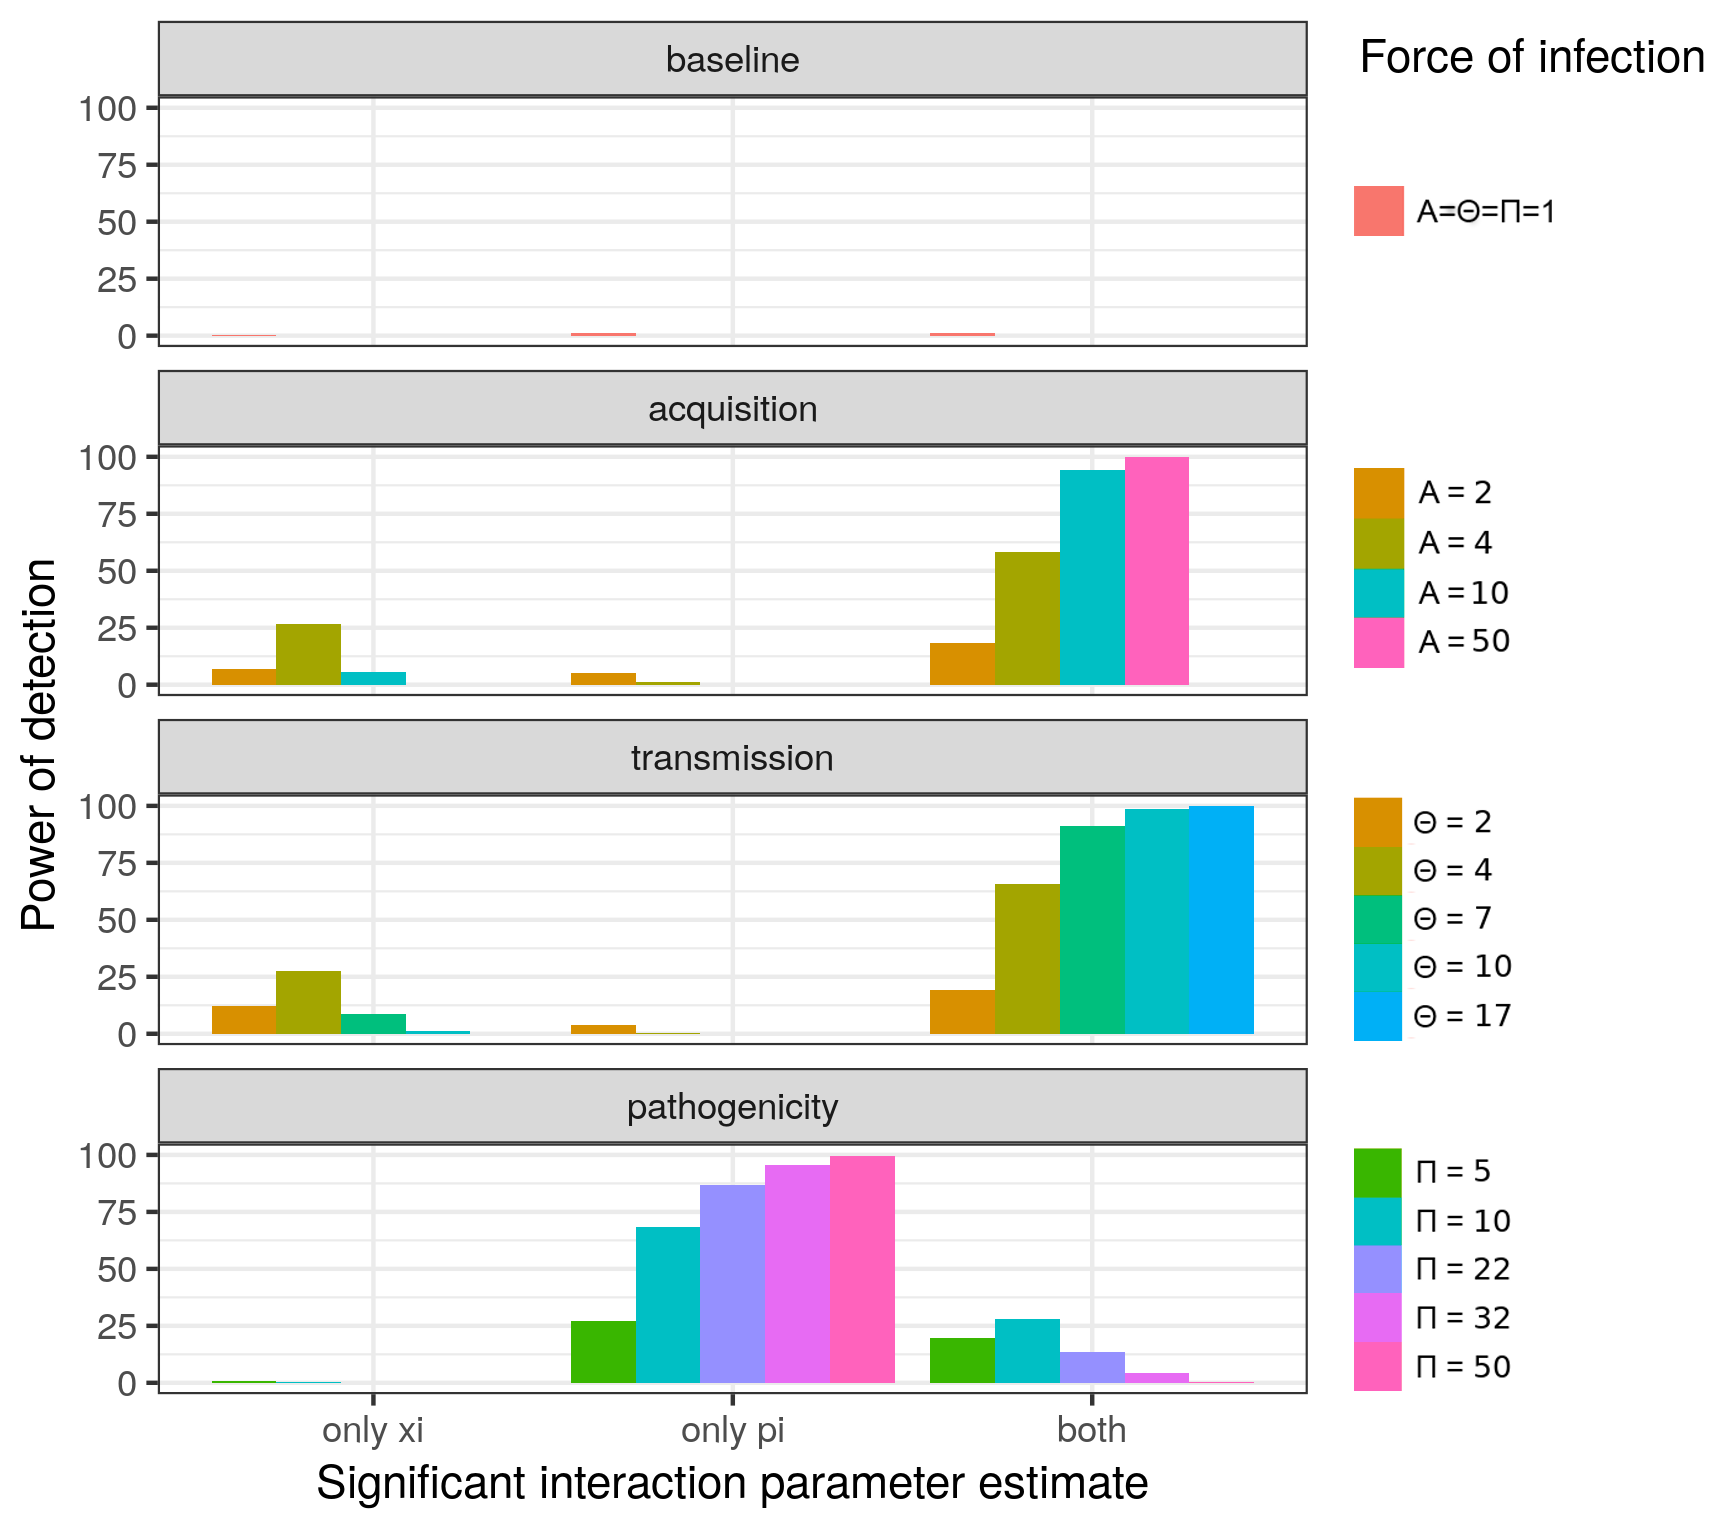
\includegraphics[width=.75\textwidth]{figures/analysis/plot_param_breakdown_power_prixThese.png}
%	\end{center}
%}



%\subsection{Conclusion}
%
%\sframe{Résultats}
%	\begin{itemize}
%		\item Toutes les méthodes
%		\begin{itemize}
%			\item seuil de détection sur la force d'interaction
%			\item importance de la saisonnalité
%			\item détection d'une association pour les mécanismes sur l'acquisition et la transmission, mais les deux mécanismes ne sont pas discernables
%		\end{itemize}
%		\medskip
%		\visible<2->{
%		\item Régressions
%		\begin{itemize}
%			\item pas d'association détectée pour le mécanisme sur la pathogénicité
%		\end{itemize}
%		}
%		\medskip
%		\visible<3->{
%		\item Modèle de transmission
%		\begin{itemize}
%			\item détection d'une association pour le mécanisme sur la pathogénicité
%			\item le mécanisme sur la pathogénicité est identifiable par rapport aux deux autres
%		\end{itemize}
%		}
%	\end{itemize}
%}



%\subsection{Synthèse}
%
%\sframe{Synthèse des valeurs estimées}
%	\begin{center}
%	
%	\includegraphics[width=.95\textwidth]{figures/analysis/synthese_reg.png}\\
%	\includegraphics[width=.95\textwidth]{figures/analysis/synthese_mod.png}
%	\end{center}
%}
%
%
%
%\subsection{Conclusion}
%
%\sframe{Conclusions}
%	\begin{itemize}
%		\item<1-> Toutes les méthodes testées sont capables de détecter une interaction dans certaines conditions
%		\begin{itemize}
%			\item Seuil de détection
%			\item Importance de la saisonnalité
%		\end{itemize}
%		\medskip
%		\item<2-> Mécanismes
%		\begin{itemize}
%			\item Régressions incapables de détecter le mécanisme sur la pathogénicité
%			\item Modélisation différencie le mécanisme sur la pathogénicité des deux autres
%		\end{itemize}
%	\end{itemize}
%}